\documentclass[12pt,a4paper]{report}
\usepackage[margin=1in]{geometry}
\usepackage{amssymb}
\usepackage{amsmath}
\usepackage{siunitx}
\usepackage{pgfplots}
\usepackage{tikz}
\usetikzlibrary{shapes,positioning,intersections,quotes}
\setlength\parindent{0pt}
\linespread{1.5}
\begin{document}

\textbf{MTHS120 Assessment 9}

\textbf{Question 1a.}

If \(g_n\), \(s_n\) and \(f_n\) are the proportions of grassland, shrubland and forest in the year \(n\) (respectively) and \(g_{n-1}\), \(s_{n-1}\) and \(f_{n-1}\) are the proportions of grassland, shrubland and forest in the year \(n-1\) (respectively), we have the following system of linear equations:

\begin{align*}
g_n &= \frac{4}{5}g_{n-1} + \frac{3}{10}f_{n-1} \\
s_n &= \frac{1}{5}g_{n-1} + \frac{9}{10}s_{n-1} + \frac{1}{10}f_{n-1} \\
f_n &= \frac{1}{10}s_{n-1} + \frac{6}{10}f_{n-1}
\end{align*} 

Represented in matrix form and using Gauss-Jordan elimination:

 \[
 \left(\begin{array}{rrr|r}
 4/5 & 0 & 3/10 & 36  \\
 1/5 & 9/10 & 1/10 & 37   \\
 0 & 1/10 & 3/5 & 27   \\
   \end{array} \right)
\] \\
 
\(R1 \rightarrow R1 \times 5/4 \)
  \[
 \left(\begin{array}{rrr|r}
 1 & 0 & 3/8 & 45   \\
 1/5 & 9/10 & 1/10 & 37   \\
 0 & 1/10 & 3/5 & 27   \\
   \end{array} \right)
\] \\
 
\(R2 \rightarrow R2 - R1 / 5 \)
  \[
 \left(\begin{array}{rrr|r}
 1 & 0 & 3/8 & 45   \\
 0 & 9/10 & 1/40 & 28   \\
 0 & 1/10 & 3/5 & 27   \\
   \end{array} \right)
\] \\
 
\(R2 \rightarrow R2 \times 10/9 \)
  \[
 \left(\begin{array}{rrr|r}
 1 & 0 & 3/8 & 45   \\
 0 & 1 & 1/36 & 280/9  \\
 0 & 1/10 & 3/5 & 27   \\
   \end{array} \right)
\] \\
 
\(R3 \rightarrow R3 - R2 / 10 \)
  \[
 \left(\begin{array}{rrr|r}
 1 & 0 & 3/8 & 45   \\
 0 & 1 & 1/36 & 280/9  \\
 0 & 0 & 43/72 & 215/9  \\
   \end{array} \right)
\] \\
 
\(R3 \rightarrow R3 \times 72/43 \)
  \[
 \left(\begin{array}{rrr|r}
 1 & 0 & 3/8 & 45   \\
 0 & 1 & 1/36 & 280/9  \\
 0 & 0 & 1 & 40   \\
   \end{array} \right)
\] \\
 
\(R1 \rightarrow R1 - R3 \times 3/8 \)
  \[
 \left(\begin{array}{rrr|r}
 1 & 0 & 0 & 30   \\
 0 & 1 & 1/36 & 280/9  \\
 0 & 0 & 1 & 40   \\
   \end{array} \right)
\] \\
 
\(R2 \rightarrow R2 - R3 / 36 \)
  \[
 \left(\begin{array}{rrr|r}
 1 & 0 & 0 & 30   \\
 0 & 1 & 0 & 30   \\
 0 & 0 & 1 & 40   \\
   \end{array} \right)
\] \\

So we can read off the values:
\begin{align*}
 g_{n-1} &= \%30 \\
 s_{n-1} &= \%30 \\
 f_{n-1} &= \%40
\end{align*} 

\newpage
\textbf{Question 1b.}

We wish to solve the following system of linear equations:
\begin{align*}
-\frac{1}{5}g_n + \frac{3}{10}f_n &= 0\\
\frac{1}{5}g_n + -\frac{1}{10}g_n + \frac{1}{10}f_n &= 0 \\
\frac{1}{10}s_n + -\frac{4}{10}f_n &= 0 \\
\end{align*} 

Represented in matrix form and using Gauss-Jordan elimination:

 \[
 \left(\begin{array}{rrr}
 -1/5 & 0 & 3/10     \\
 1/5 & -1/10 & 1/10 \\
 0 & 1/10 & -2/5  \\
    \end{array} \right)
\] \\

\(R1 \rightarrow R1 \times -5 \)
  \[
 \left(\begin{array}{rrr}
 1 & 0 & -3/2         \\
 1/5 & -1/10 & 1/10 \\
 0 & 1/10 & -2/5 \\
    \end{array} \right)
\] \\

\(R2 \rightarrow R2 -R1 / 5 \)
  \[
 \left(\begin{array}{rrr}
 1 & 0 & -3/2 \\
 0 & -1/10 & 2/5 \\
 0 & 1/10 & -2/5 \\
    \end{array} \right)
\] \\

\(R2 \rightarrow R2 \times -10 \)
  \[
 \left(\begin{array}{rrr}
 1 & 0 & -3/2 \\
 0 & 1 & -4     \\
 0 & 1/10 & -2/5 \\
    \end{array} \right)
\] \\

\(R3 \rightarrow R3 -R2 / 10 \)
 \[
 \left(\begin{array}{rrr}
 1 & 0 & -3/2 \\
 0 & 1 & -4 \\
 0 & 0 & 0      \\
   \end{array} \right)
\] \\

So the set of solutions can be expressed parametrically:
\begin{align*}
\begin{bmatrix}g_n\\s_n\\f_n\end{bmatrix} &= t \begin{bmatrix}3/2\\4\\1\end{bmatrix}
\end{align*} 


\textbf{Question 2a.}

The coefficient matrix, \( A \) is:
\[
 \left[\begin{array}{rrr}
   1 & -3 &  0 \\
   1 &  4 & -3 \\
   0 &  1 &  5 \\
   \end{array} \right] \\
\]

The determinant is:

\begin{align*}
\begin{vmatrix}
   1 & -3 &  0 \\
   1 &  4 & -3 \\
   0 &  1 &  5 \\
\end{vmatrix} &= 1 \begin{vmatrix} 4 & -3 \\
 1 & 5 \end{vmatrix} + 3 \begin{vmatrix} 1 & -3 \\ 
0 & 5 
\end{vmatrix} + 0 \begin{vmatrix} 1 & 4 \\ 
0 & 1 \end{vmatrix}\\
&= 38
\end{align*}

\textbf{Question 2b.}
\begin{align*}
\mathbf{a_1} &= (1, -3, 0) \\
\mathbf{a_2} &= (1, 4, -3) \\
\mathbf{a_3} &= (0, 1, 5) \\
\mathbf{a_1} \times \mathbf{a_3} &= (-3 \times 5 - 0 \times 1, 0 \times 0 - 1 \times 5, 1 \times 1 + 3 \times 0) \\
                                 &= (-15, -5, 1) \\
\mathbf{a_2} \times \mathbf{a_3} &= (4 \times 5 + 3 \times 1, -3 \times 0 - 1 \times 5, 1 \times 1 - 4 \times 0) \\
                                 &= (23, -5, 1) \\
\mathbf{a_1} \cdot (\mathbf{a_2} \times \mathbf{a_3}) &= (1, -3, 0) \cdot (-15, -5, 1) \\
                                                      &= 0 \\
\mathbf{a_2} \cdot (\mathbf{a_1} \times \mathbf{a_3}) &= (1, 4, -3) \cdot (23, -5, 1) \\
                                                      &= 0 \\
\end{align*}

\newpage
\textbf{Question 3a.}

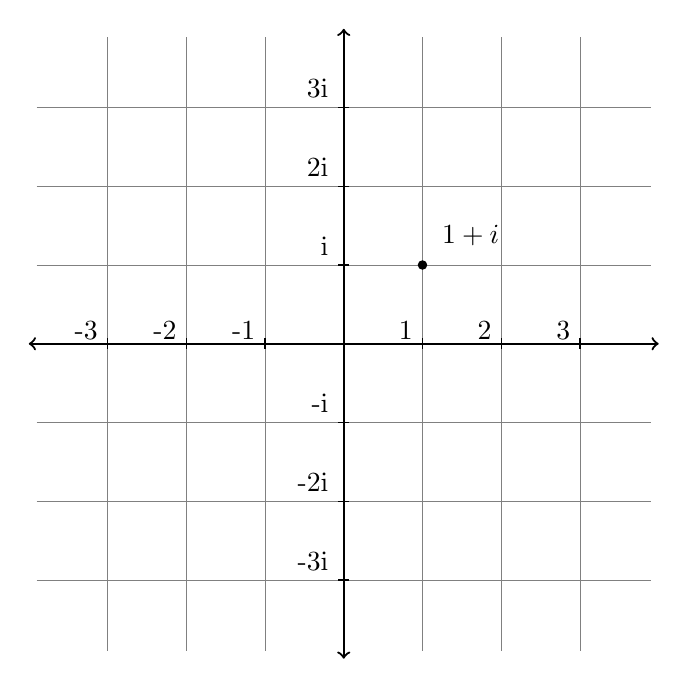
\begin{tikzpicture}
\draw[step=1cm,gray,very thin] (-3.9,-3.9) grid (3.9,3.9);
\draw[thick,->] (0,0) -- (4,0);
\draw[thick,->] (0,0) -- (0,4);
\draw[thick,->] (0,0) -- (-4,0);
\draw[thick,->] (0,0) -- (0,-4);
\draw (2pt,1) -- (-2pt,1) node[anchor=south east] {i};
\draw (2pt,2) -- (-2pt,2) node[anchor=south east] {2i};
\draw (2pt,3) -- (-2pt,3) node[anchor=south east] {3i};
\draw (2pt,-1) -- (-2pt,-1) node[anchor=south east] {-i};
\draw (2pt,-2) -- (-2pt,-2) node[anchor=south east] {-2i};
\draw (2pt,-3) -- (-2pt,-3) node[anchor=south east] {-3i};
\draw (1,2pt) -- (1,-2pt) node[anchor=south east] {1};
\draw (2,2pt) -- (2,-2pt) node[anchor=south east] {2};
\draw (3,2pt) -- (3,-2pt) node[anchor=south east] {3};
\draw (-1,2pt) -- (-1,-2pt) node[anchor=south east] {-1};
\draw (-2,2pt) -- (-2,-2pt) node[anchor=south east] {-2};
\draw (-3,2pt) -- (-3,-2pt) node[anchor=south east] {-3};
\filldraw (1,1) circle[radius=1.5pt];
\node[above right=5pt of {(1,1)}] {\(1+i\)};
\end{tikzpicture}

\begin{align*}
z &= 1 + i \\
r &= |z| \\
 &= \sqrt{1^2 + 1^2} \\
 &= \sqrt{2} \\
  \theta &= tan^{-1}(\frac{1}{1}) \\
 &= \frac{\pi}{4} \\
z &= \sqrt{2}e^{i\frac{\pi}{4}} \\
\end{align*}

\newpage
\textbf{Question 3b.}

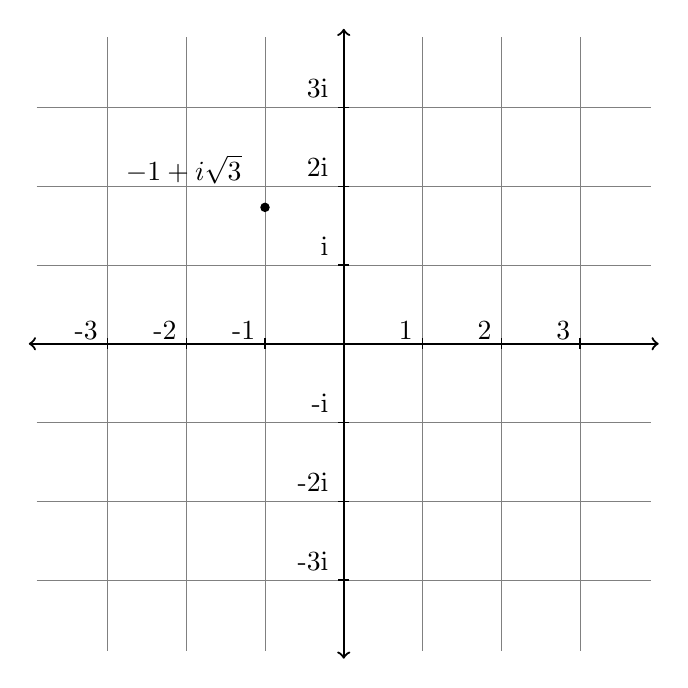
\begin{tikzpicture}
\draw[step=1cm,gray,very thin] (-3.9,-3.9) grid (3.9,3.9);
\draw[thick,->] (0,0) -- (4,0);
\draw[thick,->] (0,0) -- (0,4);
\draw[thick,->] (0,0) -- (-4,0);
\draw[thick,->] (0,0) -- (0,-4);
\draw (2pt,1) -- (-2pt,1) node[anchor=south east] {i};
\draw (2pt,2) -- (-2pt,2) node[anchor=south east] {2i};
\draw (2pt,3) -- (-2pt,3) node[anchor=south east] {3i};
\draw (2pt,-1) -- (-2pt,-1) node[anchor=south east] {-i};
\draw (2pt,-2) -- (-2pt,-2) node[anchor=south east] {-2i};
\draw (2pt,-3) -- (-2pt,-3) node[anchor=south east] {-3i};
\draw (1,2pt) -- (1,-2pt) node[anchor=south east] {1};
\draw (2,2pt) -- (2,-2pt) node[anchor=south east] {2};
\draw (3,2pt) -- (3,-2pt) node[anchor=south east] {3};
\draw (-1,2pt) -- (-1,-2pt) node[anchor=south east] {-1};
\draw (-2,2pt) -- (-2,-2pt) node[anchor=south east] {-2};
\draw (-3,2pt) -- (-3,-2pt) node[anchor=south east] {-3};
\filldraw (-1,1.732) circle[radius=1.5pt];
\node[above left=7pt of {(-1,1.732)}] {\(-1+i\sqrt{3}\)};
\end{tikzpicture}

\begin{align*}
z &= -1 + i\sqrt{3} \\
r &= |z| \\
 &= \sqrt{-1^2 + (\sqrt{3})^2} \\
 &= 2 \\
 \theta &= tan^{-1}(\frac{\sqrt{3}}{-1}) \\
 &= \frac{3\pi}{2} \quad \text{(second quadrant)} \\
 z &= 2e^{i\frac{3\pi}{2}} \\
\end{align*}

\newpage
\textbf{Question 3c.}

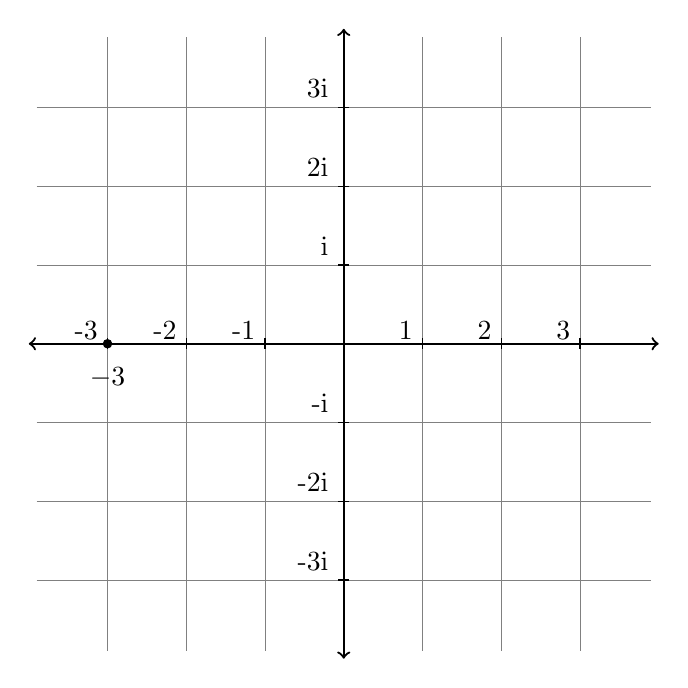
\begin{tikzpicture}
\draw[step=1cm,gray,very thin] (-3.9,-3.9) grid (3.9,3.9);
\draw[thick,->] (0,0) -- (4,0);
\draw[thick,->] (0,0) -- (0,4);
\draw[thick,->] (0,0) -- (-4,0);
\draw[thick,->] (0,0) -- (0,-4);
\draw (2pt,1) -- (-2pt,1) node[anchor=south east] {i};
\draw (2pt,2) -- (-2pt,2) node[anchor=south east] {2i};
\draw (2pt,3) -- (-2pt,3) node[anchor=south east] {3i};
\draw (2pt,-1) -- (-2pt,-1) node[anchor=south east] {-i};
\draw (2pt,-2) -- (-2pt,-2) node[anchor=south east] {-2i};
\draw (2pt,-3) -- (-2pt,-3) node[anchor=south east] {-3i};
\draw (1,2pt) -- (1,-2pt) node[anchor=south east] {1};
\draw (2,2pt) -- (2,-2pt) node[anchor=south east] {2};
\draw (3,2pt) -- (3,-2pt) node[anchor=south east] {3};
\draw (-1,2pt) -- (-1,-2pt) node[anchor=south east] {-1};
\draw (-2,2pt) -- (-2,-2pt) node[anchor=south east] {-2};
\draw (-3,2pt) -- (-3,-2pt) node[anchor=south east] {-3};
\filldraw (-3,0) circle[radius=1.5pt];
\node[below=5pt of {(-3,0)}] {\(-3\)};
\end{tikzpicture}

\begin{align*}
z &= -3 \\
r &= |z| \\
 &= \sqrt{-3^2} \\
 &= 3 \\
 \theta &= \pi \\
 z &= 3e^{i\pi} \\
\end{align*}

\textbf{Question 3c.}
\begin{align*}
 z^2 + z + 1 &= 0 \\
 z^2 + z  &= -1 \\
 z^2 + z + \frac{1}{4} &= -\frac{3}{4} \\
 (z+\frac{1}{2})^2 &= -\frac{3}{4} \\
 z+\frac{1}{2} &= \pm i\frac{\sqrt{3}}{2} \\
 z &= -\frac{1}{2} \pm i\frac{\sqrt{3}}{2} \\
 z_1 &= -\frac{1}{2} + i\frac{\sqrt{3}}{2} \\
     &= e^{i\frac{2\pi}{3}} \\
 z_2 &= -\frac{1}{2} - i\frac{\sqrt{3}}{2} \\
     &= e^{-i\frac{2\pi}{3}} \\
\end{align*}
\end{document}

